\begin{figure*}[t!]
    \centering
    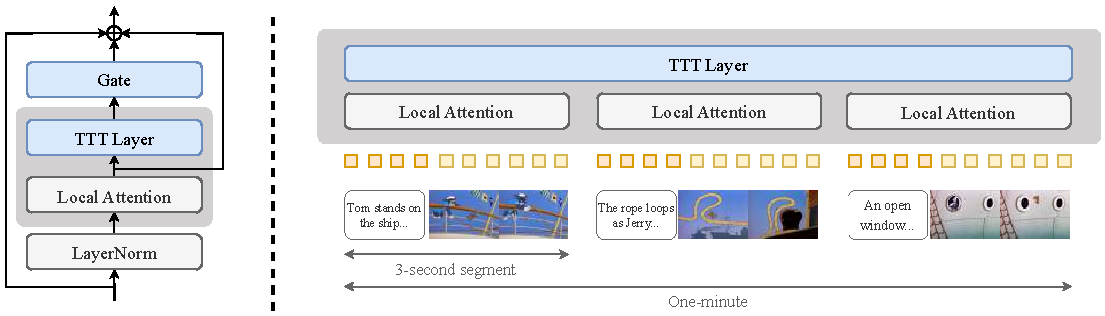
\includegraphics[width=\textwidth]{figs/integration.pdf}
    \caption{Overview of our approach. 
    \textbf{Left}: Our modified architecture adds a TTT layer with a learnable gate after each attention layer. See Subsection~\ref{subsec:arch}.
    \textbf{Right}: Our overall pipeline creates input sequences composed of 3-second segments. 
    This structure enables us to apply self-attention layers locally over segments and TTT layers globally over the entire sequence.
    See Subsection~\ref{subsec:pipeline}.}
    \label{fig:integration}
\end{figure*}

\section{Approach}
\label{sec:method}

At a high level, our approach simply adds TTT layers to a pre-trained Diffusion Transformer and fine-tunes it on long videos with text annotations. At a practical level, making this approach work involves many design choices.

\subsection{Architecture}
\label{subsec:arch}

\myparagraph{Pre-trained Diffusion Transformer.}
Our approach of adding TTT layers then fine-tuning can, in principle, work with any backbone architecture.
We choose Diffusion Transformers~\cite{peebles2023scalable} for our initial demonstration because it is the most popular architecture for video generation. 
Since the cost of pre-training a Diffusion Transformer on videos is prohibitive, we start from a pre-trained checkpoint called CogVideo-X 5B~\cite{hong2023cogvideo}.

\myparagraph{Gating.}
Given an input sequence $X = (x_1, \dots, x_T)$ where each token $x_t\in\mathbb{R}^d$, a TTT layer produces an output sequence $Z = (z_1, \dots, z_T) = \texttt{TTT}(X)$.
Each $z_t\in\mathbb{R}^d$ follows the recurrence described by Equations~\ref{eq:update_naive}, \ref{eq:multi} and \ref{eq:output} in Section~\ref{sec:prelim}.
Naively inserting TTT layers into a pre-trained network would dramatically worsen its predictions at the beginning of fine-tuning, when the TTT layers are randomly initialized.
To avoid this degradation, we gate \texttt{TTT} 
with a learned vector $\alpha\in\mathbb{R}^d$ following standard practice~\cite{alayrac2022flamingo}:
\begin{equation}
\texttt{gate}(\texttt{TTT}, X; \alpha) = \tanh(\alpha) \otimes \texttt{TTT}(X) + X,
\end{equation}
where $\tanh(\alpha)\in(-1, 1)^d$ is multiplied element-wise with each $z_t$ in $Z = \texttt{TTT}(X)$.
We initialize all values in $\alpha$ to $0.1$, so the values in $\tanh(\alpha)$ are close to 0 ($\approx 0.1$) at the beginning of fine-tuning.
This initialization of $\alpha$ allows $\texttt{TTT}$ to still contribute to $\texttt{gate}(\texttt{TTT}, X; \alpha)$ without significantly overwriting $X$.

\myparagraph{Bi-direction.}
Diffusion models, including CogVideo-X, are non-causal, meaning that an output token $z_t$ can condition on all of $x_1, \dots, x_T$ instead of only the past tokens $x_1,\dots, x_t$.
To use TTT layers in a non-causal manner, we apply a standard trick called bi-direction~\cite{mo2024scalingdiffusionmambabidirectional}. Given an operator $\texttt{rev}(X) = (x_T, \dots, x_1)$ that reverses $X = (x_1, \dots, x_T)$ in time, we define 
\begin{equation}
\texttt{TTT}'(X) = \texttt{rev}(\texttt{TTT}(\texttt{rev}(X))).
\end{equation}
Since \texttt{rev} is applied twice, $\texttt{TTT}'(X)$ is still in chronological order.
But the TTT layer inside it now scans through $X$ in reverse-chronological order.

\myparagraph{Modified architecture.}
Standard Transformers, including CogVideo-X, contain interleaving sequence modeling blocks and MLP blocks.
Specifically, a standard sequence modeling block takes an input sequence $X$ and produces
\begin{align}
X' &= \texttt{self\_attn}(\texttt{LN}(X))\label{eq:original}
\\
Y &= X' + X,
\end{align}
where \texttt{LN} is Layer Norm\footnote{Diffusion Transformers such as CogVideo-X use adaptive LN~\cite{peebles2023scalable}.} and $X' + X$ forms a residual connection.
We only modify the sequence modeling blocks, leaving everything else in the architecture unchanged. 
Each modified block, illustrated in the left panel of Figure~\ref{fig:integration}, continues from the $X'$ in Equation~\ref{eq:original} and produces
\begin{align}
Z &= \texttt{gate}(\texttt{TTT}, X'; \alpha),\label{eq:alpha}\\
Z' &= \texttt{gate}(\texttt{TTT}', Z; \beta),\label{eq:beta}\\
Y &= Z' + X.
\label{eq:modified}
\end{align}
Note that $\texttt{TTT}'$ only makes another call to \texttt{TTT}, so they share the same underlying parameters $\theta_K,\theta_V,\theta_Q$.
But for gating, Equation~\ref{eq:alpha} and~\ref{eq:beta} use different parameters $\alpha$ and $\beta$.

\subsection{Overall Pipeline}
\label{subsec:pipeline}
In this subsection, we discuss how to create the input sequence of tokens to our architecture and how each sequence is processed in segments.
Except for the first two text formats in the upcoming discussion, everything applies to both fine-tuning and inference.
Our pipeline is illustrated in the right panel of Figure \ref{fig:integration}.

\label{sec:method:pipeline}
\myparagraph{Scenes and segments.}
We structure our videos to contain multiple scenes,\footnote{
A scene is loosely defined as ``a part of a film in which the action happens in one place or is of one particular type.'' (Oxford Dictionary) 
} and each scene contains one or more 3-second \emph{segments}.
We use a 3-second segment as the atomic unit of text-to-video pairing for three reasons:
\vspace{0.2em}
\begin{itemize}[itemsep=0.2em]
\item The maximum length of generation for the original pre-trained CogVideo-X is 3 seconds.
\item The length of most scenes in the \textit{Tom and Jerry} episodes is at least 3 seconds.
\item Building a dataset with multiple stages (Subsection~\ref{subsec:dataset}) is most convenient given 3-second segments.
\end{itemize}

\myparagraph{Formats of text prompts.}
At inference time, a user can write the text prompt for a long video in any of the three formats listed below in the order of increasing detail.
See Figure~\ref{fig:prompts} in Appendix for examples of each format.
\vspace{0.2em}
\begin{itemize}[itemsep=0.2em]
    \item \textbf{Format 1}: A short summary of the plot in 5-8 sentences. Some of the examples are shown in Figure~\ref{fig:videos}.
    \item \textbf{Format 2}: A more detailed plot in roughly 20 sentences, with each sentence roughly corresponding to a 3-second segment. 
    Sentences can be labeled as belonging to certain scenes or groups of scenes, but these labels will be treated only as suggestions.
    \item \textbf{Format 3}: A storyboard. Each 3-second segment is described by a paragraph of 3-5 sentences, containing details such as background colors and camera movements. Groups of one or more paragraphs are strictly enforced as belonging to certain scenes with the keywords \mbox{\texttt{<scene start>}} and \texttt{<scene end>}.
\end{itemize}
The actual input to our text tokenizer is always in Format~3 during both fine-tuning and inference.
Conversion between the formats is performed by Claude 3.7 Sonnet in the order of $1\rightarrow2\rightarrow3$.\footnote{We observe that converting from Format 1 directly to Format 3 results in worse ability to follow the style of the human annotations in Format 3 in the fine-tuning dataset.}
For fine-tuning, our human annotations are already in Format 3, as discussed in Subsection~\ref{subsec:dataset}.

\myparagraph{From text to sequences.}
After the original CogVideo-X tokenizes the input text for each video, it concatenates the text tokens with noisy video tokens to form the input sequence to the Transformer.
To generate a long video, we apply the same procedure independently for each 3-second segment.
Specifically, given a storyboard in Format~3 with $n$ paragraphs, we first produce $n$ \emph{sequence segments}, each containing text tokens extracted from the corresponding paragraph followed by video tokens.
Then we concatenate all $n$ sequence segments together to form the input sequence, which now has interleaved text and video tokens.

\myparagraph{Local attention, global TTT.}
\mbox{CogVideo-X} uses self-attention layers to process the entire input sequence globally for each video of maximum length 3 seconds, but global attention becomes inefficient for long videos.
To avoid increasing the context length of self-attention layers, we make them local to each 3-second segment, attending to each of the $n$ sequence segments independently.\footnote{As an artifact of our pre-processing step, the sequence segments actually have an overlap of 1 latent frame (1350 tokens).}
The TTT layers process the entire input sequence globally because they are efficient in long context.

\begin{figure*}[t!]
    \centering
    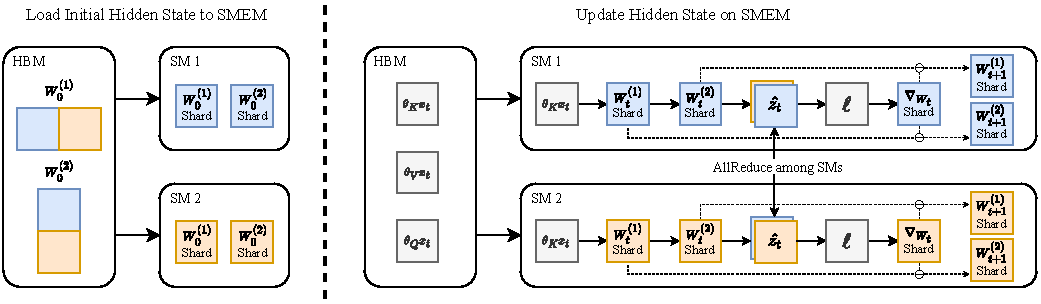
\includegraphics[width=\textwidth]{figs/systems.pdf}
    \caption{On-chip Tensor Parallel, discussed in Subsection~\ref{subsec:gpu}.
    \textbf{Left:} To reduce the memory required on each SM for TTT-MLP, we shard the hidden state $W^{(1)}$ and $W^{(2)}$ across SMs, transferring them between HBM and SMEM only during initial loading and final output.
    \textbf{Right:} We update the hidden state entirely on-chip and use the DSMEM feature on the NVIDIA Hopper GPU architecture to \texttt{AllReduce} intermediate activations among SMs.
    }
    \label{fig:sys}
\end{figure*}

\subsection{Fine-Tuning Recipe and Dataset}
\label{subsec:dataset}

\myparagraph{Multi-stage context extension.}
Following standard practice for LLMs~\cite{xiong2023effective}, we extend the context length of our modified architecture to one minute in five stages.
First, we fine-tune the entire pre-trained model on 3-second segments of \textit{Tom and Jerry} to adapt it to this domain.
New parameters (specifically those in TTT layers and gates) are assigned a higher learning rate during this stage.
Over the next four stages, we fine-tune on videos of 9, 18, 30, and eventually 63 seconds.
To avoid forgetting too much of the world knowledge from pre-training,
we only fine-tune the TTT layers, gates, and self-attention layers, using a lower learning rate during these four stages. 
See Appendix~\ref{sec:appendix:implementation} for the detailed recipe.

\myparagraph{Super-resolution on original videos.}
We start with 81 episodes of \textit{Tom and Jerry} released between 1940 and 1948.
Each episode is about 5 minutes, adding up to about 7 hours for all episodes.
The original videos vary in resolution, which is uniformly poor by modern standards.
We run a video super-resolution model~\cite{wang2021realesrgan} on the original videos, producing visually enhanced videos with shared resolution of $720\times480$ for our dataset.

\myparagraph{Multi-stage dataset.}
Following the structure discussed in Subsection~\ref{subsec:pipeline}, we first have human annotators break down each episode into scenes, then extract 3-second segments from each scene.
Next we have human annotators write a detailed paragraph for each 3-second segment.\footnote{
Each paragraph includes 1–2 sentences describing the background, 1–2 sentences describing the characters, and 2 sentences describing actions and camera movements. 
On average, each paragraph contains 98 words, which corresponds to 132 tokens.
}
Stage~1 fine-tunes directly on these segments.
To create data for the last four stages, we concatenate contiguous 3-second segments into videos of 9, 18, 30 and 63 seconds together with their text annotations.
Scene boundaries are marked by the same keywords in Subsection~\ref{subsec:pipeline}. As a result, annotations for all training videos are in Format~3.

\subsection{Parallelization for Non-Causal Sequences}
\label{subsec:parallel}
The update rule discussed in Section~\ref{sec:prelim} cannot be naively parallelized across tokens in a sequence, since computing $W_t$ requires $\nabla\ell(W_{t-1}; x_t)$, which in turn requires $W_{t-1}$.
To enable parallelization, we update $W$ on $b$ tokens at a time, which \cite{sun2024ttt} calls an inner-loop mini-batch.
Throughout this paper, we set $b=64$.

Concretely,  
for mini-batch $i = 1,\dots,T/b$ (assuming $T$ is an integer multiple of $b$), 
\begin{equation}
W_{ib} = W_{(i-1)b} - \frac{\eta}{b}\sum_{t=(i-1)b+1}^{ib}\nabla \ell\left(W_{(i-1)b}; x_t\right).
\label{eq:ttt_update_new}
\end{equation}
Because the sequence is non-causal, we then use $W_{ib}$ to produce the output tokens for all timesteps in mini-batch $i$:
\begin{equation}
    z_t = f(W_{ib}; x_t), \quad \quad \text{for}~~t = (i-1)b+1,\dots, ib.
    \label{eq:ttt_output_new}
\end{equation}
Note that $W_{(i-1)b+1},\dots,W_{ib-1}$ are no longer needed.

After this modification, $f$ can process an (inner-loop) mini-batch of tokens in parallel, similar to how a regular MLP processes an (outer-loop) mini-batch of training data. 
As a side benefit, we observe that averaging gradients across tokens reduces variance and stabilizes each update to $W$.

\subsection{On-Chip Tensor Parallel}
\label{subsec:gpu}
Implementing TTT-MLP efficiently for GPUs requires special designs to take advantage of their memory hierarchy.
A chip on a GPU is called a Streaming Multiprocessor (SM), analogous to a core on a CPU.
All SMs on a GPU share a relatively slow but large global memory called HBM, 
then each SM has a fast but small on-chip memory called SMEM.
Frequent data transfers between the SMEMs and HBM on a GPU can significantly hurt overall efficiency.

Efficient implementations of Mamba and self-attention layers (Flash Attention~\cite{dao2022flashattention}) use kernel fusion to minimize this kind of transfer. 
The high-level idea of these implementations is to load inputs and initial states into each SMEM, perform computations entirely on-chip, and write only the final outputs back to HBM. 
However, the hidden state for TTT-MLP, namely the weights $W^{(1)}$ and $W^{(2)}$ of the two-layer MLP $f$, is too large to be stored in the SMEM of a single SM (when combined with inputs and activations).

To reduce the memory required on each SM, we use Tensor Parallelism~\cite{shoeybi2019megatron} to shard $W^{(1)}$ and $W^{(2)}$ across SMs, as shown in Figure \ref{fig:sys}. 
Similar to how large MLP layers can be sharded and trained across the HBMs of multiple GPUs, 
we apply the same idea now across the SMEMs of multiple SMs, treating each SM as the analogy of a GPU. 
We use the DSMEM feature on the NVIDIA Hopper GPU architecture to implement \texttt{AllReduce} among SMs.
More details of our kernel are discussed in Appendix~\ref{sec:appendix:systems}.

Our implementation significantly improves efficiency, since hidden states and activations are now read from and written to HBMs only during initial loading and final output.
As a general principle, if a model architecture $f$ can be sharded with standard Tensor Parallelism across GPUs, then the same sharding strategy can be applied across SMs when $f$ is used as the hidden state.